
\section{Regular Expression}
% ======================================================================

\subsection{Regular Language}
%----------------------------------------------------------------------

We've learned that the class of regular language is closed under
\begin{compactitem}
\item union,
    \footnote{
    $
    \text{ if } L_1, L_2 \in \mathbb R,
    \text{ then }
    L_1 \cup L_2 = \set{ w \mid w \in L_1 \lor w \in L_2 }
    \in \mathbb R
    .$
    }
\item intersection,
    \footnote{
    $
    \text{ if } L_1, L_2 \in \mathbb R,
    \text{ then }
    L_1 \cap L_2 = \set{ w \mid w \in L_1 \land w \in L_2 }
    \in \mathbb R
    .$
    }
\item concatenation, and
    \footnote{
        $
        \text{ if } L_1, L_2 \in \mathbb R,
        \text{ then }
        L_1 \cdot L_2 = \set{ w_1w_2 \mid w_1 \in L_1 \land w_2 \in L_2 }
        \in \mathbb R
        .$
    }
\item star.
    \footnote{
        \label{ftnote:star_operation}
        $
        \text{ if } L \in \mathbb R,
        \text{ then }
        L^* = \set{ w_1w_2 \cdots w_n \mid w_1,w_2, \cdots, W_n \in L, n \ge 0 }
        \in \mathbb R
        .$
    }
\end{compactitem}

\begin{example}[Build a rather complex language using * operation]
    It is common we want to search for all numbers, say, in a file. The following set is a
    language that matches all numbers greater than $10$ and allowing appearance of commas.
    \[
        L =
        \set{1,\cdots,9} \cdot
        \( \set{0,1,\cdots,9}^* \cdot \set{,} \)^* \cdot
        \set{0,1,\cdots,9}
    \]

    Consider 
    \begin{align*}
        L_1 = \set{1,\cdots,9} \\
        L_2 = \set{0,1,\cdots,9}^* \cdot \set{,}  \\
        L_3 = \set{0,1,\cdots,9}  \\
    \end{align*}
    so 
    $L = L_1 \cdot L_2^* \cdot L_3$.

    What are $L_1$, $L_2$ and $L_3$?
    \begin{compactdesc}
    \item[$L_1$] is a set of all digits from $1$ to $9$;
    \item[$L_3$] is a set of all digits from $0$ to $9$;
    \item[$L_2$] is a little more complicated, it can also be written as $L_3^* \cdot
        \set{,}$, while $L_3^*$ matches a string of any number of elements in $L_3$, that
        is, a string made of all digits with unknown length. What $\cdot \set{,}$ does is
        it appends a comma to the end of this string. In all, $L_2$ is a number of digits
        with a comma at the end.
    \end{compactdesc}

    With that, the set $L_1 \cdot L_2^* \cdot L_3$ can be now (roughly) seen as:
    \[
        a\ digit \text{ and }
        a\ number\ of ( a\ number\ of\ digits \text{ and } a\ comma ) \text{ and }
        a\ digit
    \]
    Now, notice there is a leading digit and an ending one, why should one be in $L_1$ and
    the other $L_3$? Because matching from set $L_1$ rules out the numbers with leading
    $0$s ($L_1$ doesn't have $0$), and the rest of digits should allow $0$s. The middle
    portion ($L_2^*$) allows unknown number of strings from $L_2$ (even $0$) in between
    the first and last digit. In the case where the number of $L_2$ is $0$, which makes
    the input string also in set $L_1 \cdot L_3$, the input string is a two-digit number
    ($10$ to $99$).
\end{example}

\begin{example}[$\mathbb R$ closed under star (see footnote\ref{ftnote:star_operation})]
    We have a regular language $A_1$ and want to prove that ${A_1}^*$ also is regular.
    \begin{proof} \ \\
        We take an NFA $N_1$ for $A_1$ and modify if to $N$ to recognize ${A_1}^*$.

        We can construct $N$ like $N_1$ with additional $\varepsilon$ arrows returning to
        the start state from the accept states. This way, when processing gets to th end
        of a piece that $N_1$ accepts, the machine $N$ has the option of jumping back to
        the start state to try to read in another piece that $N_1$ accepts.

        We also need to add a new sart state and make it an accept state, and which has an
        $\varepsilon$ arrow to the old start state. So it accept empty string $\varepsilon
        (n = 0)$.
        
        See the graph for visualization:
        \begin{center}
            \begin{minipage}{2.5cm}
                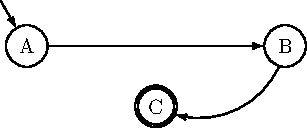
\includegraphics[width=\textwidth]{pics/mp/nfa-7.pdf}
                \center $N_1$
            \end{minipage}
            \; $\longrightarrow$ \;
            \begin{minipage}{3.5cm}
                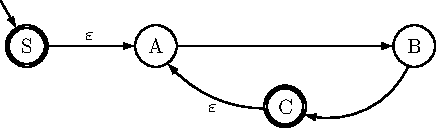
\includegraphics[width=\textwidth]{pics/mp/nfa-8.pdf}
                \center $N$
            \end{minipage}
        \end{center}

        One bad idea is simply to make original start state to final state. This approach
        certainly adds $\varepsilon$ to the recognized language, but it may also add
        other, undesired stings.

    \end{proof}
\end{example}

\subsection{Regular Expression}
% ----------------------------------------------------------------------

A regular expression (abbreviated regex or regexp) is a sequence of characters that forms
a search pattern, mainly for use in pattern matching with strings, or string matching.
(via \href{http://en.wikipedia.org/wiki/Regular_expression}{WikiPedia})

A regex $E$ can be transformed to language of DFA as follow
\begin{align*}
    & E = a                   && L(a) = \set{a}                        \\
    & E = \varepsilon         && L(\varepsilon) = \set{\varepsilon}    \\
    & E = E_1 \cdot E_2       && L(E) = L(E_1) \cdot L(E_2)            \\
    & E = E_1 + E_2           && L(E) = L(E_1) + L(E_2)                \\
    & E = (E_1)^*             && L(E) = L\((E_1)^*\) = L(E_1)^*        \\
    & E = \varnothing         && L(\varnothing^*)
\end{align*}
In fact, the rule
\[
    L(\varepsilon) = \set{\varepsilon}
\]
can be replaced with 
\[
    L(\varnothing^*).
\]

\begin{theorem}[Equivalence of Regex and Regular Language]
    \[
        \forall L \in \mathbb R,
        \exists \text{ Regex } E \text{ s.t.\ } L(E) = L.
    \]
\end{theorem}

\subsection{GNFA}
% --------------------------------------------------

A generalized nondeterministic finite automaton (GNFA) is an NFA where
\begin{compactitem}
\item there are exactly one arrow entering and one leaving a state,
\item states can be transited using regexes ($\varnothing$ arrows, star arrows, etc.),
\item there are no arrows entering the initial state,
\item there is only one final state, and
\item there are no arrows leaving the final state.
\item there are no arrows entering the start state.
\end{compactitem}

\begin{definition}[GNFA]
    A GNFA is defined as a $5$-tuple
    \[
        \lst{ Q,\Sigma,\delta,s,f }
    \]
    where
    \[
        \delta \colon
        (Q - \set{q_{\text{accept}}}) \times (Q - \set{q_{\text{start}}})
        \mapsto
        \mathbb R(\Sigma)
    \]
\end{definition}

A GNFA, since it can use transitions with regexes, can help develop a regex of the
language of the GNFA 

To translate a NFA to a GNFA:
\begin{compactenum}
\item add a new start state with $\varepsilon$ arrow connect to its odd start state, 
\item removing states one at a time until we have the form
    \centgraph[3.5cm]{pics/mp/gnfa-0}
\item make $\set{q \in f}$ to non-accept states, connect those original final states to a
    new and unique final state.
\end{compactenum}

\bigskip

The concept of regex finely relates to all automata we've learned so far:
\centgraph[3cm]{pics/mp/relation_automata_regex-0}

The general translation will be as follow:
RegEx $ \Rightarrow $ NFA $ \Rightarrow $ DFA $ \Rightarrow $ NFA $ \Rightarrow $ GNFA $
\Rightarrow $ RegEx

